
\chapter{Sinn und Zweck paralleler Programmierung}
\label{intro}
Seit Beginn der Rechentechnik Anfang der 40er Jahre verfolgen Informatiker das Ziel die zur Verfügung stehende Rechenleistung effizient zu nutzen.

Die parallele Programmierung stellt eine wesentliche Maßnahme dar, um dieses Ziel zu erreichen. Mit dieser Arbeit  soll die Umsetzung eines gegebenen Problems auf einer Grafikkarte mittels nVidia CUDA vorgestellt werden.

Parallele Programme beschreiben potentiell gleichzeitig ablaufende Aktivitäten, die miteinander kooperieren, um eine gemeinsame Aufgabe zu lösen. Dies setzt Programme voraus, die unabhängig von der Anzahl und der Geschwindigkeit der Prozessoren die gewünschten Ergebnisse liefern. Die Softwareentwicklung für parallele Algorithmen ist deshalb im Vergleich zur sequentiellen Programmierung wesentlich komplexer.

Durch die Aufteilung eines Programms in sogenannte \textbf{Threads} (\glqq leichtgewichtige Prozesse\grqq) lassen sich die Ressourcen heutiger Mirkoprozessoren effizient nutzen.
Threads besitzen dabei folgende Eigenschaften:
\begin{itemize}
\item sind sequentielle Befehlsausführungen
\item stellen Einheit für die Prozessorzuteilung dar
\item laufen in einem Prozessadressraum ab
\end{itemize}
Mit der Einführung von Threads werden im wesentlichen zwei Ziele verfolgt:
\begin{enumerate}
\item Strukturierung unabhängiger Programme und Programmkomponenten
\item Leistungssteigerung durch effiziente Parallelarbeit
\end{enumerate}

%Besonders aus der Möglichkeit der effizienten Parallelarbeit geht ein weiterer wesentlicher Vorteil hervor:
Die Leistungsfähigkeit von Programmen ist hauptsächlich abhängig von der Taktrate der CPU. Erhöht sich die Taktrate, wird ebenso das Programm schneller.
Allerdings haben die Taktraten heutiger CPUs einen Grenzwert erreicht.
Größere Taktraten würden diverse technische Probleme mit sich bringen, wie beispielsweise erhöhte Wärmeentwicklung auf dem Prozessor und damit verbundene, eine geeignete Wärmeabfuhr zu finden.
Daher gehen Chiphersteller schon seit einigen Jahren den Weg, möglichst viele Recheneinheiten (Kerne) auf einer CPU unterzubringen. Grafikprozessoren sind von Haus aus mit einer deutlich größeren Anzahl an Kernen ausgestattet.
Programme die entsprechend implementiert wurde diese Technologien effizient zu nutzen, können einen deutlichen Geschwindigkeitsvorteil gegenüber einer parallelen Ausführung auf einer CPU aufweisen.


\chapter{Aufgabenstellung}
Gegeben Kraft-Abstandskurven eines Rasterkraftmikroskops. Rasterkraftmikroskope werden zur Untersuchung von Oberflächen genutzt, um bspw. ein Höhenprofil erstellen zu können. Hierzu wird die vorliegende Oberfläche an möglichst vielen Stellen mit einer ca. 40 nm großen Spitze abgetastet, d.h. es wird zu jeder Messhöhe die der Abtastspitze entgegengebrachte Kraft gemessen.
Der Verlauf einer solchen Kraft-Abstandskurve lässt sich in drei lineare Funktionen unterteilen und ist qualitativ in Abbildung \ref{fig:kraftqual} dargestellt.

\begin{figure}[h!]
\centering
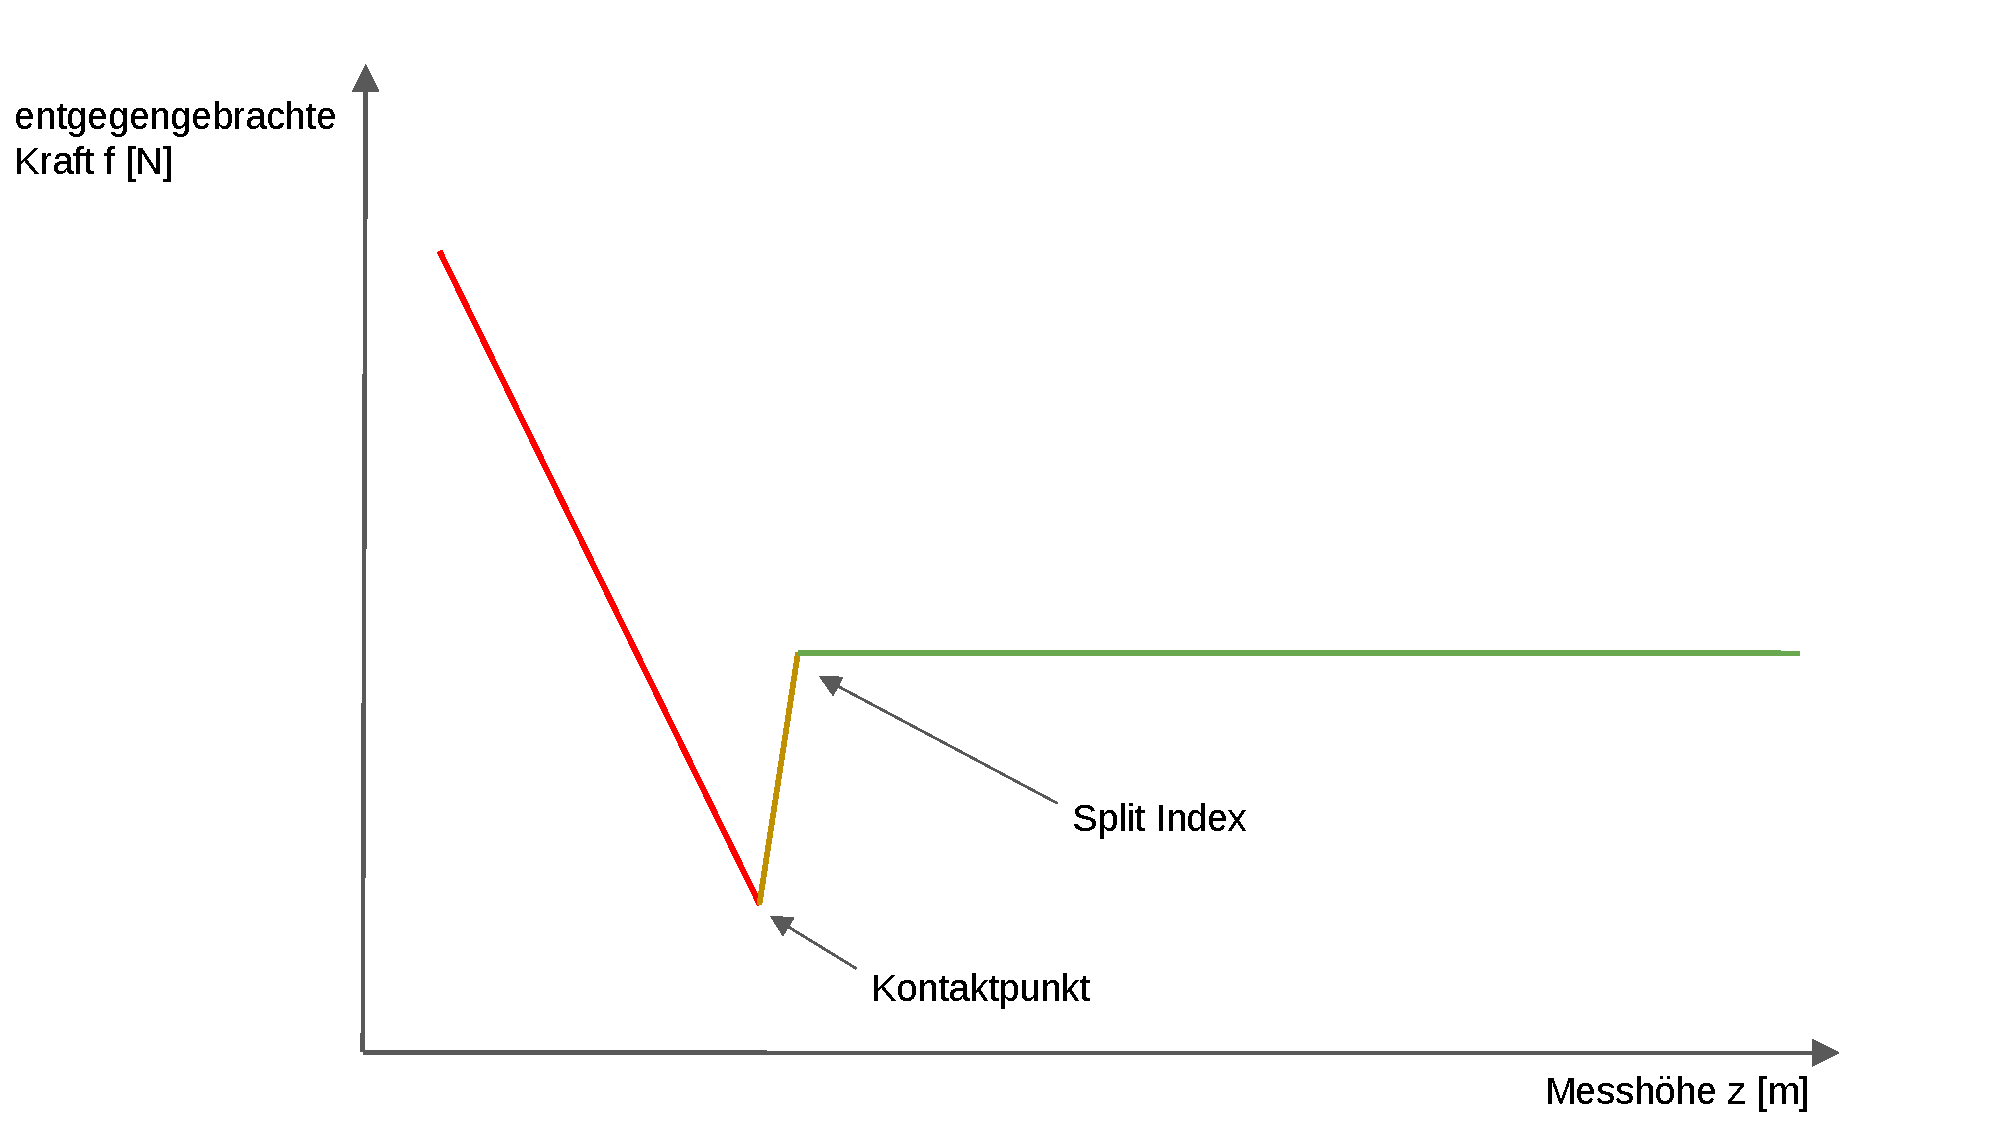
\includegraphics[scale=0.5]{qual.pdf}
\caption{Qualitativer Verlauf einer Kraft-Abstandskurve}
\label{fig:kraftqual}
\end{figure}

Der grüne Kurvenverlauf stellt die Annäherung der Abtastspitze zur Probe dar. Auffällig ist, dass die entgegengebrachte Kraft bei diesem Vorgang konstant bleibt.
Die gelbe Kurve zeigt, wie die Spitze von den Adhäsionskraften zwischen ihr und der Probe erfasst wird. Die entgegengebrachte Kraft fällt daher rapide ab, bis die Spitze Kontakt mit der Probe an der Stelle $c$ hergestellt hat.
Der rote Kurvenabschnitt zeigt, wie die auf die Spitze einwirkende Kraft nach Kontaktherstellung stark zunimmt, während weiterhin versucht wird, sich der Probe anzunähern.

Ziel ist es nun, die gegebene Punktewolke eines realen Rasterkraftmikroskops in diese drei linearen Funktionen zu zerlegen.
Ein Ausschnitt einer solchen realen Kraft-Abstandskurve ist in Abbildung \ref{fig:kraftbsp} dargestellt.


\begin{figure}[h!]
\centering
 \begin{tikzpicture}[scale=1]
 \begin{axis}[
   width=15cm,
   xlabel=Messhöhe in m,
   ylabel=Kraft in N]
 \addplot table [y=$Q_A$, x=P]{ex.txt};
 %\addlegendentry{$Q_A$ series}
 \end{axis}
 \end{tikzpicture}
\caption{Ausschnitt einer Kraft-Abstandskurve}
\label{fig:kraftbsp}
\end{figure}

Aufgenommen wurden solche Abtastungen an 256x*256y Positionen, wobei sowohl eine Messung für das Anfahren auf die Probe als auch das Ablassen von ihr aufgezeichnet wurde. Es liegen also insgesamt 131072 Datensätze vor, deren je 300 Abtastwerte mittels dreifach linearer Regression auf einer GPU in die oben beschriebene Form gebracht werden sollen, indem der Kontaktpunkt mit der Probe und der Splitindex gefunden werden.


\section{Einlesen der Datensätze}
\label{einlesen}
Die Datensätze liegen als Textdeateien vor, wobei an jede Messposition in einer eigenen Datei gepsiechert ist. Es liegen somit 65536 Textdateien vor, in denen die Messwerte für das An-/ und Abfahren von der Probe zeilenweise ähnlich wie in einer CSV Datei gepseichert sind.
Das Einlesen dieser vielen 100KiB kleinen Dateien wird durch das häufige öffnen und schließen der Dateien und dem damit verbundenen Overhead seitens des Betreibssystems verlangsamt. Zudem werden für die nötigen Berechnungen nur die ersten zwei der insgesamt 14 Datenspalten benötigt, was Caching seitens des OS zusätzlich erschwert.


Das Einlesen aller 65536 Textdateien benötigt auf einer SSD\footnote{Testsystem: openSUSE 13.2, Linux Kernel 3.16.7 x86\_64, OCZ Vertex 3} 2 Minuten. Dies kann auf 40 Sekunden reduziert werden, wenn das Einlesen mittels openMP Tasks parallelisiert erfolgt.
Der Einlesevorgang auf einer konventionellen HDD benötigt aufgrund der trägen Mechanik hingegen mind. 10 Minuten.

Um dies zu umgehen ist eine Vorverarbeitung nötig, die darin besteht, die Textdateien einmalig einzulesen, die Daten zu filtern und zu sortieren und sie anschließend als Binär Blob auszugeben. Der Einlesevorgang kann somit auf wenige Sekunden reduziert werden.

\section{Implementierung des Kernels}
Als Eingabe erhält der Kernel die aus dem Binär Blob gelesenen Datensätze.
Der Kernel hat die Aufgabe die Eingangs beschriebene dreifache lineare Regression für jeden Datensatz durchzuführen.

\begin{lstlisting}[caption=Implementierung des Kernel in Pseudocode,label=kernel]
void kernel(const point_t* pts, const int nSets)
{
    int myAddr = threadIdx.x+blockIdx.x*blockDim.x;

    if(myAddr < nSets)
    {
        const my_size_t nPoints = pts[myAddr].n;

        contactIdx = calcContactPoint(pts[0:nPoints])
        __syncthreads();

        fitPoints(pts[0:contactIdx]);
        __syncthreads();
                
        my_size_t splitIdx = contactIdx+10;
        fitPoints(pts[contactIdx:splitIdx]);

        fitPoints(pts[splitIdx:nPoints]);
    }
}
\end{lstlisting}


Aufgrund der vergleichsweise geringen Anzahl an Messwerten pro Datensätze (=300) erfolgt eine naive Parallelisierung der Datensätze: Jeder Thread der Grafikkarte bearbeitet einen Datensatz. Wie in Codelisting \ref{kernel} dargestellt wird hierfür

\begin{itemize}
\item die gegebene Punktwolke abgeleitet, um den Kontaktpunkt zu bestimmen (Zeile 7),
\item eine lineare Regression (polyfit) der Kurve vom Ende der Messung bis zum Kontakt mit dem Medium durchgeführt (Zeile 12),
\item der Split-Index erraten\footnote{Die Berechnung des Split-Indexes erwies sich als zu aufwendig und instabil, daher wurde auf eine Implementierung im Rahmen dieses Seminars verzichtet.} (Zeile 15),
\item ein polyfit der Kurve zwischen dem Kontaktpunkt bis Split-Index  (Zeile 16) und
\item ein polyfit der Kurve zwischen Split-Index und Anfang der Messung durchgeführt  (Zeile 18).
\end{itemize}

Grafikkarten arbeiten im SIMD Verfahren. Um zu verhindern, dass die Threads divergieren, da sich die Kontaktpunkte und die Länge der zu interpolierenden Kurve zwangsläufig zwischen den Datensätzen unterscheiden, wurde in den Zeilen 10 und 13 Synchronisationsbarrieren auf Thread-Block Ebene eingeführt.
Diese konnten in der Praxis jedoch keine messbare Veränderung der Laufzeit hervorbringen, da bei nur 300 Messwerten pro Datensatz eine mögliche Divergenz der GPU-Threads zu gering ist.

\section{Datenmodell}
Um eine effiziente Verarbeitung auf der Grafikkarte zu erreichen, müssen die Datensätze in geeigneter Weise strukturiert werden.
Dazu muss entschieden werden, ob sie Daten als \gls{aos} oder als \gls{soa} übergeben werden. Nachfolgend werden diese Ansätze diskutiert.

\subsection{\acrlong{aos}}
\begin{lstlisting}[label=aos_row,caption=\gls{aos} row major]
struct tuple_t { float z,f; };
tuple_t datasets[M][N];
\end{lstlisting}

%N: anzahl an datensätze
%M: anzahl an messwerten pro datensatz

Die Auslegung der Daten als \gls{aos} bedeutet, dass die Daten als zweidimensionales Array übergeben werden, deren Element ein Verbunddatentyp ist, welcher die gemessene Kraft f an der entsprechenden Messhöhe z enthält. Wird das Array wie in Listing \ref{aos_row} dargestellt row major im Speicher abgelegt, Liegen die N Datensätze zeilenweise im Speicher, sodass die i-te Speicherzeile die M Messwerte des i-ten Datensatzes enthält.
Dies ist jedoch für Grafikkarten ungeeignet, da die Messwerte für die einzelnen Threads zu weit auseinander liegen. D.h. wird eine Cacheline geladen, kann hiervon nur das erste Element (der erste Messwert) verwendet werden. Die anderen Threads benötigen ebenfalls den ersten Messwert allerdings den des ihnen zugeordneten Datensatzes. Diese befinden sich in anderen Zeilen des Speichers.
Es müssen somit weitere Cachelines geladen werden, was schlimmsten falls zu einer Ausserialisierung der Threads führt.


\begin{lstlisting}[label=aos_col,caption=\gls{aos} column major]
struct tuple_t { float z,f; };
tuple_t datasets[N][M];
\end{lstlisting}

Es empfiehlt sich daher die Datensätze column major im Speicher abzulegen, wie in Listing \ref{aos_col} dargestellt. Die i-te Zeile des Speichers enthält somit die i-ten Messwerte aller Datensätze. Da jeder Thread einen Datensatz bearbeitet, können alle 32 Threads eines Warps durch eine Cacheline mit Daten versorgt werden.


\subsection{\acrlong{soa}}
Bei NVidia Grafikkarten vor der Pascal Architektur erhält jeder Thread durch einen Lesevorgang ein 32 bit Wort aus der Cacheline\footnote{\href{http://docs.nvidia.com/cuda/pascal-tuning-guide/index.html\#shared-memory-bandwidth}{http://docs.nvidia.com/cuda/pascal-tuning-guide/index.html\#shared-memory-bandwidth}}. tuple\_t hat jedoch eine Größe von 8 Bytes. 
Es braucht also zwei Lesevorgänge um alle Threads eines Warps mit Daten zu versorgen.
Um einen Performancevergleich zu der älteren Kepler Architektur zu erhalten, wird daher auch eine \gls{soa} Variante, wie in Listing \ref{soa} dargestellt, implementiert.
%daher folgende Optimierung:

\begin{lstlisting}[label=soa,caption=\gls{soa}]
struct tuple_t { float z[N],f[N]; };
tuple_t datasets[M];
\end{lstlisting}

Hier ist tuple\_t ein reines \gls{soa}, welches M mal existiert und jeweils Zeiger auf Arrays enthält, welche die N Messwerte z und f des jeweiligen Datensatzes enthalten. Diese können somit von N Threads single strided bearbeitet werden, wie schematisch in Listing \ref{soa_beispiel} dargestellt.
Zwar hat tuple\_t nun eine Größe von 16 Byte, da es zwei 8 Byte Zeiger enthält. Dieses Element muss jedoch nur einmalig gelesen werden, da die enthaltenen Zeiger von den N Threads gemeinsam verwendet werden können.

\begin{lstlisting}[label=soa_beispiel,caption=Bearbeitung eines \gls{soa}]
tuple_t datasets[M];
extern int threadId;

for (i=0; i<M; i++)
{
    float myZ = datasets[i].z[threadId];
    float myForce = datasets[i].f[threadId];
    
    // doWork(myZ, myForce);
}
\end{lstlisting}


\chapter{Benchmarking}
%\section{lesen der textdateien}
%von konventioneller HDD: 8MiB/s
%von SSD:  35 MiB/s -O0
%70 MiB/s -O2
%41 s bei 190 MiB/s -O2 paralleles lesen mit openmp tasks
%
%referenz implementierung 11 MiB/s von SSD
%
%referenz implementierung 11 minuten insgesamt


\section{Berechnung}
Eine in Python geschriebene Referenzimplementierung diente als Vorlage für die im Rahmen dieses Seminars erstellte C++ Implementierung. Sie bearbeitet die Datensätze seriell auf der CPU und benötigt dafür insgesamt 11 Minuten.

Die C++ Implementierung benötigt die für die in Abschnitt \ref{einlesen} beschriebene Vorverarbeitung der Datensätze 40 Sekunden. Parallel verarbeitet werden die Datensätze schnellstenfalls in ca. 250 Millisekunden. Da die C++ Implementierung verglichen zur Referenzimplementierung aus Zeitgründen jedoch unvollständig ist, nehmen wir für die Berechnung des Speedups 1 Sekunde Bearbeitungszeit auf der CPU an.

Der Speedup beider Implementierungen auf der CPU beträgt somit.

$S = \dfrac{T_{seriell}}{T_{parallel}} = \dfrac{11*60}{40+1} = 16$

65536*2 Datensätze:
AoS Ansatz: GPU: 3.5 ms CPU Single: 545 ms CPU 4HWThreads: 199 ms
SOA Ansatz: GPU: 2.27 ms CPU: ??

benchmarking mit double? verdoppelt zeit da wir genug double precision units haben aber eben zwei cachlines lesen müssen anstatt von nur einer

\section{CPU vs. GPU bei variierender Problemgröße}


NVidia GeForce GTX 1060: 1280 HW-Threads; 6GB GDDR5
Intel Core i5-3570K: 3.40 GHz; 4 HW-Threads

\begin{figure}[]
\centering
 \begin{tikzpicture}[scale=1]
 \begin{axis}[
   width=15cm,
   legend style={at={(0,1)},anchor=north west},
   /pgf/number format/.cd,
   use comma,
   1000 sep={},
   xlabel=Anzahl Datensätze,xmode = log,log basis x={2},ymode = log,log basis y={2},
   ylabel=Berechnungszeit in ms]
 \addplot table [x=N,y=Kaos]{test_privat};
  \addplot table [x=N,y=Ksoa]{test_privat};
   \addplot table [x=N,y=Caos]{test_privat};
    \addplot table [x=N,y=Csoa]{test_privat};
    \addplot table [x=N,y=cpy]{test_privat};
    \legend{GPU Kernel AoS,GPU Kernel SoA,CPU AoS, CPU SoA, cudaMemcpy}
    
 %\addlegendentry{$Q_A$ series}
 \end{axis}
 \end{tikzpicture}
~\\~\\
 \pgfplotstabletypeset[
columns/N/.style={/pgf/number format/fixed, /pgf/number format/.cd,use comma,1000 sep={}},
columns/Kaos/.style={column name={GPU Kernel AoS},/pgf/number format/.cd,use comma,1000 sep={}},
columns/Ksoa/.style={column name={GPU Kernel SoA},/pgf/number format/.cd,use comma,1000 sep={}},
columns/Caos/.style={column name={CPU AoS},/pgf/number format/.cd,use comma,1000 sep={}},
columns/Csoa/.style={column name={CPU SoA},/pgf/number format/.cd,use comma,1000 sep={}},
columns/cpy/.style={column name={cudaMemcpy},/pgf/number format/.cd,use comma,1000 sep={}}
]{test_privat}
\caption{Benchmark CPU vs. GPU auf Privatrechner}
\label{fig:benchmark:privat}
\end{figure}


Die Berechnungszeiten steigen erwartungsgemäß linear zur Problemgröße an. Die GPU ist jedoch mit 27 ms bei $2^{20}$ Datensätzen deutlich schneller als die CPU mit bestenfalls 2,8 s. Überraschend ist auch, dass der \gls{soa} mit dem \gls{aos} Ansatz auf der GPU nahezu gleich auf liegt. Eine auf der Pascal Architektur erwartete Präferenz für den \gls{aos} Ansatz ist zwar leicht vorhanden, grenzt sich jedoch mit einem Unterschied von 5 ms bei $2^{20}$ Datensätzen nur unwesentlich vom \gls{soa} Ansatz ab.
Erkennbar ist dass der Zugriff auf den Grafikkartenspeicher bei der Pacsal-Architektur optimiert wurde. Dennoch bleibt die PCI-E Schnittstelle ein Flaschenhals.

Zu beobachten ist auch, dass die \gls{soa} Variante auf der CPU erst ab $2^{18}$ Datensätzen besser performt als \gls{aos}. Diese Beobachtung deckt sich mit dem Benchmark auf gpu03, siehe Abbildung \ref{fig:benchmark:gpu03}.


\begin{figure}[]
\centering
 \begin{tikzpicture}[scale=1]
 \begin{axis}[
   width=15cm,
   legend style={at={(0,1)},anchor=north west},
   /pgf/number format/.cd,
   use comma,
   1000 sep={},
   xlabel=Anzahl Datensätze,xmode = log,log basis x={2},ymode = log,log basis y={2},
   ylabel=Berechnungszeit in ms]
 \addplot table [x=N,y=Kaos]{test_gpu03};
  \addplot table [x=N,y=Ksoa]{test_gpu03};
   \addplot table [x=N,y=Caos]{test_gpu03};
    \addplot table [x=N,y=Csoa]{test_gpu03};
    \addplot table [x=N,y=cpy]{test_gpu03};
    \legend{GPU Kernel AoS,GPU Kernel SoA,CPU AoS, CPU SoA, cudaMemcpy}
    
 %\addlegendentry{$Q_A$ series}
 \end{axis}
 \end{tikzpicture}
 ~\\~\\
  \pgfplotstabletypeset[
columns/N/.style={/pgf/number format/fixed, /pgf/number format/.cd,use comma,1000 sep={}},
columns/Kaos/.style={column name={GPU Kernel AoS},/pgf/number format/.cd,use comma,1000 sep={}},
columns/Ksoa/.style={column name={GPU Kernel SoA},/pgf/number format/.cd,use comma,1000 sep={}},
columns/Caos/.style={column name={CPU AoS},/pgf/number format/.cd,use comma,1000 sep={}},
columns/Csoa/.style={column name={CPU SoA},/pgf/number format/.cd,use comma,1000 sep={}},
columns/cpy/.style={column name={cudaMemcpy},/pgf/number format/.cd,use comma,1000 sep={}}
]{test_gpu03}
\caption{Benchmark CPU vs. GPU auf gpu03.inf-ra.uni-jena.de}
\label{fig:benchmark:gpu03}
\end{figure}


Die beiden Peaks bei $2^{10}$ Datensätzen auf dem Privatrechner und bei $2^{17}$ auf gpu03 lassen sich durch Cache-Assoziativität-Effekte erklären. Normalerweise entscheidet die Speicheradresse eines Datums in welchen Teil des Caches sie abgelegt werden. Bei den erwähnten Peaks scheinen die Arrays unter den CPU Threads so ungünstig aufgeteilt zu sein, dass die Daten der einzelnen Threads aufgrund ähnlicher Speicheradressen immer an die gleiche Stelle im Cache geschrieben werden. Der Cache wird somit künstlich verkleinert und es kommt vermehrt zu Cachemisses.

%Diese Vermutung bestätigt sich durch die Wahl des dynamischen schedules, bei dem eine ungleichmäßige Aufteilung des Arrays unter den Threads erfolgt. Das hierbei entstehende Benchmark ist in Abbildung \ref{fig:benchmark:privat:dynamic} dargestellt.
%
%
%\begin{figure}[h!]
%\centering
% \begin{tikzpicture}[scale=1]
% \begin{axis}[
%   width=15cm,
%   legend style={at={(0,1)},anchor=north west},
%   /pgf/number format/.cd,
%   use comma,
%   1000 sep={},
%   xlabel=Anzahl Datensätze,xmode = log,log basis x={2},ymode = log,log basis y={2},
%   ylabel=Berechnungszeit in ms]
% \addplot table [x=N,y=Kaos]{test_privat_dynamic};
%  \addplot table [x=N,y=Ksoa]{test_privat_dynamic};
%   \addplot table [x=N,y=Caos]{test_privat_dynamic};
%    \addplot table [x=N,y=Csoa]{test_privat_dynamic};
%    \legend{GPU Kernel AoS,GPU Kernel SoA,CPU AoS, CPU SoA}
%    
% %\addlegendentry{$Q_A$ series}
% \end{axis}
% \end{tikzpicture}
%\caption{Benchmark CPU vs. GPU auf Privatrechner (dynamic schedule)}
%\label{fig:benchmark:privat:dynamic}
%\end{figure}
%
%
%\begin{figure}[h!]
%\centering
% \begin{tikzpicture}[scale=1]
% \begin{axis}[
%   width=15cm,
%   legend style={at={(0,1)},anchor=north west},
%   /pgf/number format/.cd,
%   use comma,
%   1000 sep={},
%   xlabel=Anzahl Datensätze,xmode = log,log basis x={2},ymode = log,log basis y={2},
%   ylabel=Berechnungszeit in ms]
% \addplot table [x=N,y=Kaos]{test_gpu03_dynamic};
%  \addplot table [x=N,y=Ksoa]{test_gpu03_dynamic};
%   \addplot table [x=N,y=Caos]{test_gpu03_dynamic};
%    \addplot table [x=N,y=Csoa]{test_gpu03_dynamic};
%    \legend{GPU Kernel AoS,GPU Kernel SoA,CPU AoS, CPU SoA}
%    
% %\addlegendentry{$Q_A$ series}
% \end{axis}
% \end{tikzpicture}
%\caption{Benchmark CPU vs. GPU auf gpu03 (dynamic schedule)}
%\label{fig:benchmark:privat:dynamic}
%\end{figure}


\chapter{Fazit}
Die durchgeführten Tests haben gezeigt, dass sich die von Rasterelektronenmikroskopen aufgenommenen Kraft-Abstands-Messungen performant auf modernen Grafikkarten verarbeiten lassen.
Ein nicht zu vernachlässigender Overhead stellt jedoch der Kopiervorgang der Datensätze auf den Grafikkartenspeicher dar. Eine tatsächliche Implementierung auf einer Grafikkarte würde sich erst dann bezahlt machen, wenn mit den vorhandenen Daten noch mehr Berechnungen durchgeführt werden würde, als die hier beispielhaft implementierte dreifach lineare Regression. Oder aber wenn, wie in den Benchmarks gezeigt, die Anzahl der Datensätze statt der vorhandenen $2^{17}$ beträchtlich (d.h. gegen $2^{20}$ und mehr) gesteigert werden würde.
Anderenfalls wird der zusätzlich benötigte Entwicklungsaufwand auf einer Grafikkarte nicht gerechtfertigt, da auch ältere CPUs mit 4 Rechenkernen $2^{20}$ Datensätze in weniger als 3 Sekunden bearbeitet haben.